%% Public domain image from
%% http://www.public-domain-image.com/objects/computer-chips/slides/six-computers-chips-circuits.html
\renewcommand\chapterillustration{OGL_transform/chapterImage}



\chapter{OpenGL의 변환}

\index{변환!OpenGL}

\index{변환!OpenGL}\index{transformation}\index{어파인 변환}\index{affine transformation}
수학에서 변환(transformation)이란 어떤 집합 $S$를 다른 어떤 집합 혹은 자기 자신 $S$로 대응시키는 함수를 의미한다. 이러한 변환은 하나의 기하 객체를 다른 위치로 옮겨 놓는 작용을 하게 된다. 따라서 그래픽스에서는 물체를 옮겨 놓는 데에 변환을 활용한다. 앞서 2차원 도형을 이용하여 집, 산, 나무 등을 두 개의 원을 그렸다.
하나는 하늘에 뜬 해이고 다른 하나는 나무의 잎을 표현하였다.
이때 두 원은 중심점의 위치가 다르고 반지름도 다르다. 이 반지름과 중심점을 이용하여
우리가 그리려고 하는 원의 정점(vertex)들을 서로 다른 코드를 이용하여 따로 생성하였다.
그런데 변환을 이용하면 이런 문제를 좀 더 단순하게 만들 수 있다. 


\section{OpenGL에서의 변환}

우선 앞에서 살펴본 두 개의 원 그리리기 문제를 다시 생각해 보자.
그리고 어떤 기하객체를 옮기고, 모양을 바꾸는 변환을 우리가 자유자재로 할 수 있다고 하자.
이때 좌표를 이동시키는 변환을 $T()$라고 하고, 
크기를 변경하는 변환을 $S()$라고 하면, 우리에게 필요한 그리기 함수는 반지름 1인 원 그리기 하나면 충분하다.
이 그리기를 $draw()$라고 하자. 그러면 다음과 같은 방식으로 다양한 원을 원하는 곳에 원하는 크기로 그릴 수 있다.

\begin{verbatim}
T ( S(draw(), scale), displacement)
\end{verbatim}

이렇게 변환을 활용할 수 있다면, 원을 그리는 코드는 두 번 다 따로 작성할 필요 없이 한 번의 구현만으로 충분하다.
변환은 다양한 방식으로 이루어질 수 있다. 이 절에서는 OpenGL과 같은 실시간 그래픽 라이브러리에서 변환을 어떻게 다루며, 
그래픽스 프로그래밍에서 어떻게 활용할 수 있는지를 다룰 것이다.

\subsection{어파인(affine) 변환}
어파인(affine)은 서로 연결되어 있음을 의미하는 라틴어 `affinis'에서 온 말이다. 어파인 변환은 직선 위의 점들을 직선을 유지한 상태로 변환하는 변환이며, 직선 위에서의 점들 사이의 거리 비가 변환된 직선 위에서 그대로 유지되는 변환이다. 이런 특성에 의해 직선은 직선으로, 평행선은 평행선으로 유지된다. 이러한 어파인 변화의 예가 그림 \ref{fig:OGL_transform:affineXform}에 있다.

\begin{figure}[h!]
  \centering
    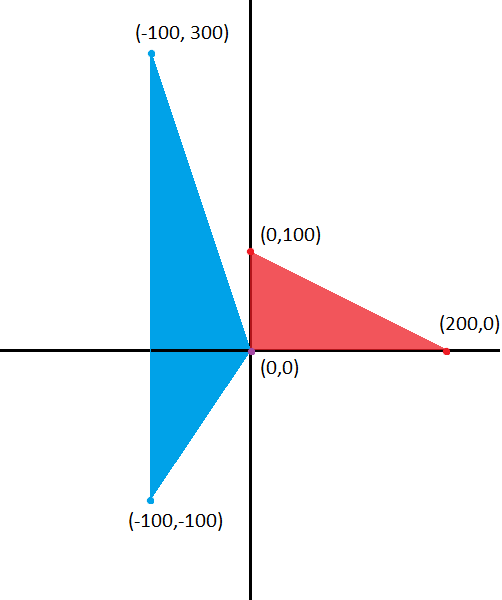
\includegraphics[height=8cm]{OGL_transform/affineXform.png}
    \caption{어파인 변환의 예}
    \label{fig:OGL_transform:affineXform}
\end{figure}

OpenGL이나 DirectX와 같은 실시간 그래픽스 라이브러리에서는 기하 객체를 표현할 때, 일반적으로 하나의 면을 구성하는 정점과 이 정점들에 의해 정의되는 면을 화소별로 표현하는 프래그먼트로 구분한다. 프래그먼트의 특성은 정점의 특성을 선형보간하여 얻는다. 직선이 직선으로 옮겨지는 affine 변환의 특성을 고려할 때, 변환이 적용되는 대상은 각 면의 정점만으로 충분하다. 정점들을 연결하는 선이나 내부를 구성하는 프래그먼트는 변환에 영향을 받지 않고 마찬가지의 방법으로 구성할 수 있다. 따라서 실시간 그래픽스 라이브러리에서는 일반적으로 어파인 변환만을 사용한다. 대표적인 어파인 변환은 표 \ref{tab:transform:affineXforms}과 같다.

\begin{table}
\caption{대표적인 어파인 변환의 예}
\label{tab:transform:affineXforms}
\begin{center}
    \begin{tabular}{ |l| p{10cm} |}
    \hline
    {\small \sf 이동(translate)} & {\small \sf 주어진 변위 벡터만큼 좌표를 동일하게 옮겨 놓는다.} \\ \hline
    {\small \sf 회전(rotate)} & {\small \sf 2차원에서는 기준점, 3차원에서는 기준축을 중심으로 주어진 각도만큼 돌아간다.}\\ \hline
    {\small \sf 크기변경(scale)} & {\small \sf 각 축 방향으로 주어진 비율에 따라 좌표 값이 커지거나 줄어든다.}\\ \hline
    \hline
    \end{tabular}
\end{center}
\end{table}


\subsection{동차좌표(homogenous coordinate)}\index{동차좌표계}\index{homogeneous coordinate}

동차 좌표(homogeneous coordinate)은 $n$ 차원의 사영공간을 $n+1$ 차원의 좌표로 나타내는 좌표계를 의미한다.
동차좌표계 혹은 사영좌표계(projective coordinates)는 1827년 아우구스트 페르디난드 뫼비우스(August Ferdinand M\"{o}bius)가 그의 저작 ``Der barycentrische Cal\"{u}l"에서 처음으로 소개하였다. 유클리드 기하에서 사용되는 데카르트 좌표계(Cartesian coordinate)와 달리 사영기하학에서 사용되는 좌표계이다. 이 좌표계는 무한의 위치에 있는 점을 유한 좌표로 표현하는 데에 적합하다.

3차원 공간의 기하 좌표를 세 개의 숫자로 표현하는 방식을 사용할 경우 이동은 벡터의 덧셈으로 표현되고, 회전은 $3 \times 3$ 행렬의 곱으로 표현된다. 따라서 이동과 회전이 누적되면 벡터 덧셈과 행렬 곱셈이 연속적으로 일어나게 된다. 그런데, 동차좌표(homogeneous coordinate)을 사용하면 이동과 회전 모두 $4 \times 4$ 행렬의 곱으로 표현할 수 있다. 따라서 누적된 이동, 회전 변환을 하나의 행렬로 표현할 수 있게 된다.
이러한 이유로 3차원 컴퓨터 그래픽스에서 좌표는 4 개의 숫자를 가진 동차좌표를 사용하고, 변환은 4 $\times x$ 4의 행렬로 표현하는 것이다.


\subsection{OpenGL에서의 변환}\index{변환 행렬}\index{transform matrix}
동차 좌표계에서 어파인 변환은 행렬로 표현된다. 일반적으로 실시간 그래픽스에서는 affine 변환만을 사용하기 때문에 OpenGL 역시 변환을 행렬로 표현한다. OpenGL은 정점 데이터를 그래픽 카드로 보내는데, 각각의 정점들은 필요한 변환 행렬에 곱해져서 최종적인 화면 좌표를 가지게 된다. 이때 곱해지는 행렬이 두 종류가 있는데 하나는 모델뷰(ModelView) 행렬이며, 다른 하나는 투영(Projection) 행렬이다. 모델뷰 행렬은 물체를 3차원 공간 내에서 이동, 회전 시키는 변환을 담고 있으며, 3차원 공간의 좌표를 2차원 평면에 어떻게 떨어뜨릴 것인지를 결정하는 변환행렬이 투영행렬이다. 하나의 정점이 화면 좌표로 바뀌는 과정은 다음과 같다. 지역좌표계 내의 좌표를 $coord_{local}$이라고 하고, 모델뷰 행렬은 $ModelViewMatrix$, 투영행렬을 $ProjMatrix$라고 하며, 화면 좌표 $coord_{screen}$은 다음과 같이 구한다.
\index{투영행렬}\index{projection matrix}\index{모델뷰 행렬}\index{modelview matrix}

$$coord_{screen} = ProjMatrix  \times ModelViewMatrix \times coord_{local}$$

OpenGL의 변환은 이 행렬들을 변경하는 것이라고 할 수 있다. 모델 뷰 행렬을 바꿀 것인지 혹은 투영 행렬을 바꿀 것인지는 행렬 모드에 의해 결정된다. 각각의 행렬에 해당하는 모드는 {\sf GL\_MODELVIEW}와 {\sf GL\_PROJECTION}이 있다. OpenGL에서 사용하는 행렬은 몇 가지가 더 있지만 현재로서는 이 두 가지만을 고려하자.
우선 투영 행렬을 변경하는 방식은 카메라의 속성을 변경하는 것으로 앞에서 살펴본 {\sf glOrtho}나 {\sf gluPerspective}와 같은 함수들을 적용하는 것이다. 이것은 카메라에 해당되는 것이기 때문에 여기서는 설명을 하지 않겠다. 우선은 앞서 살펴본 간단한 카메라 설정 정도의 지식만 가지고 시작하자.

모델뷰 행렬을 변경하는 함수는 이미 간단한 카메라 조작에서 살펴본 {\sf gluLookAt} 같은 함수가 있다. 사실 OpenGL은 어떤 경우에도 카메라가 원점에 존재한다. 그러면 {\sf gluLookAt}은 어떻게 카메라를 원하는 위치로 옮길 수 있는지 의문스러울 것이다. 사실 {\sf gluLookAt}은 카메라를 원하는 곳에 원하는 방향으로 두는 것이 아니라, 동일한 효과를 갖도롤 모든 물체를 카메라의 움직임과 반대로 움직여 두는 것이다. 결국 카메라는 언제나 원점에서 $z$ 축 음의 방향을 쳐다보고 있다.

다음으로 공간내의 물체들을 움직이고 회전시키는 변환은 표 \ref{tab:transform:OpenGLXforms}과 같은 것들이 있다.

\begin{table}
\caption{OpenGL에서 사용하는 대표적인 변환}
\label{tab:transform:OpenGLXforms}
\begin{center}
    \begin{tabular}{ |l| p{8cm} |}
    \hline
    {\small \sf glTranslate3f(dx, dy, dz);} & {\small \sf (dx,dy,dz) 만큼 좌표 이동} \\ \hline
    {\small \sf glRotatef(angle, axisX, axisY, axisZ);} & {\small \sf 축(axisX, axisY, axisZ)를 기준으로 angle만큼 회전}\\ \hline
    {\small \sf glScalef(scaleX, scaleY, scaleZ);} & {\small \sf  (scaleX, scaleY, scaleZ)를 성분별로 좌표에 곱함}\\ \hline
    \hline
    \end{tabular}
\end{center}
\end{table}
이상의 변환들은 좌표를 실제로 변경하지 않고 현재의 행렬을 변경하는 역할을 수행한다. 즉 현재의 행렬이 $\bf M$이라고 하고, {\sf glTranslate}의 이동을 표현하는 행렬이 $\bf T$라고 하자. OpenGL은 {\sf glTranslate} 함수가 불렸을 때, $\bf M$을 $\bf MT$로 변경한다. 

\subsection{현재 변환 행렬(current transformation matrix)}
현재 변환 행렬은 줄여서 CTM이라 부르며, 모든 정점은 이 CTM에 곱해진다. 따라서 앞서 살펴본 변환 함수는 이 CTM을 변경하는 것이다.
이 CTM을 변경하는 함수로 다음과 같은 것들이 있고, 이들이 CTM을 바꾸는 방식은 표 \ref{tab:transform:CTM}과 같다.\\


\begin{table}
\caption{적용된 변환에 따른 CTM의 변화 과정}
\label{tab:transform:CTM}
\begin{tabular}{|c|p{10cm}|}\hline
{\small \sf 함수 } & {\small \sf CTM의 변경}\\ \hline
{\small \sf LoadIdentity} & {\small \sf CTM := I}\\ \hline
{\small \sf LoadMatrix(M)} & {\small \sf CTM := M}\\ \hline
{\small \sf T: Translate*} & {\small \sf CTM := CTM * T}\\ \hline
{\small \sf R: Rotate*} & {\small \sf CTM := CTM * R}\\ \hline
{\small \sf S: Scale*}	& {\small \sf CTM := CTM * S}\\ \hline
\end{tabular}
\end{table}

예를 들어 다음의 코드 \ref{code:OGL_transform:transform}과 같이 변환이 적용될 경우 
CTM은 이 코드에 주석 처리된 부분에 나타난 것과 같이 변경이 된다.
이 코드에서는 CTM을 단위행렬 $\mathbf I$로 초기한다.
그리고 {\sf glTranslate, glRotate, glScale}를 이용하여
각각 ${\mathbf T, \mathbf R, \mathbf S}$를 만든다. 이 행렬들은 기존의 CTM에 만들어진 순서에 따라
오른쪽에 곱해진다. 다시 말해 어떤 정점이 주어지만
${\mathbf S, \mathbf R, \mathbf T}$의 순서로 적용되는 것이다.



\begin{algorithmbis}[변환의 적용에 따른 CTM의 변화]\label{code:OGL_transform:transform}
\lstset{language=C++, escapechar=^} 
\begin{lstlisting}
glMatrixMode(GL_MODELVIEW);
glLoadIdentity();			// CTM:=I
glTranslatef(1,2,1);		// CTM:=IT ^{\it T는 glTranslate가 표현하는 행렬}^
glRotatef(45, 1,0,0);		// CTM:=ITR ^{\it R은 glRotate가 표현하는 행렬}^
glScalef(2.0, 1.0, 1.0);	// CTM:=ITRS ^{\it S는 glScale이 표현하는 행렬}^
drawObjects();
\end{lstlisting}
\end{algorithmbis}

코드 \ref{code:OGL_transform:transform}은 drawObjects 내에서 그려지는 모든 기하 객체의 좌표에 대해 크기변환($\mathbf S$)을 적용한 뒤, 이 값을 $x$ 축 기준으로 45도 회전하게 되며, 이후 (1,2,1) 만큼의 이동을 한다. 다시말해 우리가 호출한 변환의 역순으로 변환이 객체에 적용된다. 
다음 코드 \ref{code:OGL_transform:translate}를 살펴보자.

\begin{algorithmbis}[이동 변환의 적용]\label{code:OGL_transform:translate}
\lstset{language=C++, escapechar=^} 
\begin{lstlisting}
void draw() {
    glutWireSphere(0.5, 30, 30); // ^{\it 반지름 0.5의 구를 원점을 중심으로 그림}^
}
void display() {
    ^{\sf [[여기에 카메라 설정(gluLookAt 등), 버퍼 클리어(glClear) 코드]]}^
    drawAxes(); // ^{\it 축을 그림}^
    glColor3f(1, 1, 0);
    draw(); // ^{\it 아무런 변환 없이 원점에 구를 그림}^
    glTranslatef(1.0, 0.0, 0.0); //^{\it $(1,0,0)$ 벡터만큼 이동을 함}^
    glColor3f(0, 1, 1);
    draw(); //^{\it 적용된 변환을 이용하여 구를 그림}^
    glTranslatef(-0.5, 1.0, 0.0); //^{\it $(-0.5,1,0)$ 벡터만큼 이동을 함}^
    glColor3f(1, 0, 0);
    draw(); //^{\it 적용된 변환을 이용하여 옮겨진 구름 그림}^
    glutSwapBuffers();
}
\end{lstlisting}
\end{algorithmbis}

\begin{figure}[h!]
  \centering
    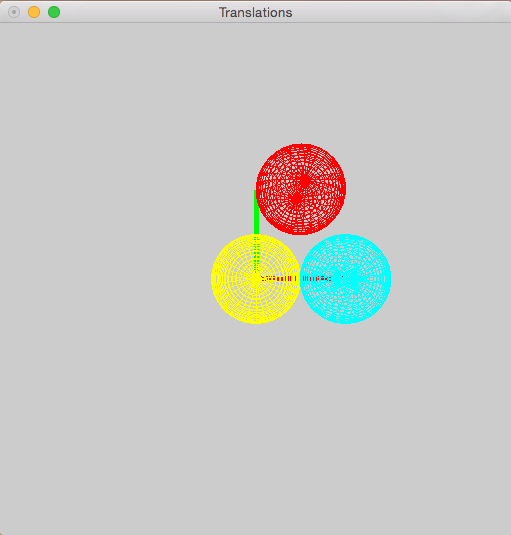
\includegraphics[height=7cm]{OGL_transform/transformedBalls.png}
    \caption{변환에 의해 서로 다른 위치에 놓인 구(sphere)들}
    \label{fig:OGL_transform:transformedBalls}
\end{figure}

노란 색, 하늘 색, 붉은 색 공이 차례로 그려진다.  노란 색 공에는 변환이 적용되지 않았으므로 원점에 그려지고, 하늘 색 공에는 (1,1,0) 만큼의 이동이 적용된다. 마지막 붉은 색 공은 (-0.5, 1, 0)의 변환이 적용된 후에 하늘 색에 적용된 (1,1,0) 만큼의 이동이 추가되어 전체적으로 (0.5, 1, 0)의 위치에 그려진다. 이상과 같이 이동은 이해하기 쉽다. 결과는 그림. \ref{fig:OGL_transform:transformedBalls}과 같다.







\section{복합 변환의 이해}
\index{복합 변환}
OpenGL을 이용하여 변환을 수행하는 함수를 누적하여 호출한 경우, 실제 객체에 적용되는 변환은 호출 순서의 역으로 적용된다는 것을 살펴 보았다.
이것은 앞선 절에서 살펴본 바와 같이 CTM을 활용한 변환 적용 기법을 사용하기 때문이다. 그런데, 이러한 방식으로 변환의 적용을 이해하면 매우 적용된 변환을 상상하기가 쉽지 않고, 원하는 변환을 코드(code)로 구현하는 것이 까다롭다. 그림 \ref{fig:OGL_transform:fourTeapots}과 같이 네 개의 주전자를 배치하고 싶다고 하자. 이를 OpenGL로 구현하려면 어떻게 해야할 지를 고민해 보자. 이 절의 내용은 이를 쉽게 할 수 있는 능력을 갖추는 것이다.

\begin{figure}[h!]
  \centering
    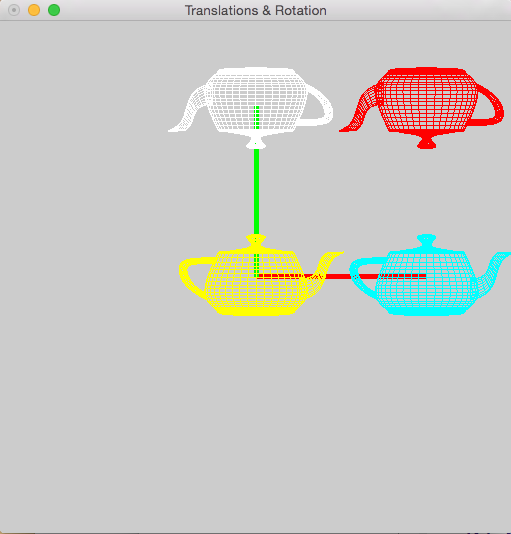
\includegraphics[height=7cm]{OGL_transform/fourTeapots.png}
    \caption{서로 다른 위치에 서로 다른 방향으로 놓인 주전자들}
    \label{fig:OGL_transform:fourTeapots}
\end{figure}


\subsection{CTM 모델로 원하는 변환 구현해 보기}

노란색, 하늘색, 붉은색, 흰색 주전자의 순서로 그린다고 가정해 보자. 주전자를 그리는 함수를 {\sf draw(color)}라고 가정하자.
노란색 주전자는 아무런 변환도 적용되지 않은 상태이다. 따라서 아무 변환 함수 호출 없이 바로 그리면 된다.

\begin{verbatim}
glLoadIdentity();
draw(yellow);				// CTM = I 
\end{verbatim}

다음으로 하늘색 주전자는 $x$ 축으로 1만큼 이동하여 그려야 하므로 {\sf glTranslate*} 함수를 부른 뒤 주전자를 그린다. 이때 불린 이동 변환을 T1이라고 하자.

\begin{verbatim}
glTranslatef(1.0, 0.0, 0.0);  // T1
draw(cyan);
\end{verbatim}

다음으로 붉은 색 주전자를 보자. 이 주전자는 $z$ 축을 기준으로 180도 회전한 뒤에 (1,1,0)만큼 이동한 것이다. 현재의 CTM이 ${\mathbf T}_1$, 
즉 (1,0,0)만큼의 이동이므로 (0,1,0)만큼의 이동 ${\mathbf T}_2$를 추가 적용하면 (1,1,0) 이동이 되며, 여기에 회전 ${\mathbf R}$을 적용한다.

\begin{verbatim}
glTranslate(0.0, 1.0, 0.0);		// T2
glRotatef(180, 0.0, 0.0, 1.0);	// R
draw(red);
\end{verbatim}

이러면 붉은 색 주전자는${\mathbf T}_1 {\mathbf T}_2  {\mathbf R}$의 변환을 적용받게 된다. 
즉, $z$ 축 기준 180도 회전 ($\mathbf R$)을 적용한 뒤, 앞서 호출된 (1,1,0) 만큼의 이동 (${\mathbf T}_1 {\mathbf T}_2$)를 수행한다.
여기서 마지막 흰색 주전자를 그리는 방법은 다소 까다롭니다. 이 주전자는 180도 회전 시킨 주전자를 (0,1,0) 만큼 이동한 것인데, 
현재의 변환에서 어떤 변환을 추가적으로 호출하면 이것이 가능할지 생각해 보자. 
지금까지의 변환이 이동만 있다면 붉은색 주전자를 그리듯이 쉽게 다음 변환 함수를 생각할 수 있지만, 이미 회전이 호출된 상태라 까다롭다.
새롭게 적용할 변환이 $\mathbf  X$라고 하고, (0,1,0) 만큼 이동하는 변환을 ${\mathbf T}$라고 하면 다음과 같은 관계가 된다.

이 X는 다음과 같다.

위의 계산을 수행하면 X는 (1,0,0) 만큼의 이동으로 나타나게 된다. 따라서 다음과 같이 적용하면 원하는 결과를 얻을 수 있다.

\begin{verbatim}
glTranslatef(1.0, 0.0, 0.0);	// X
draw(white);
\end{verbatim}

이런 방식으로 ${\mathbf  X}$를 결정하여 다음 변환을 부르는 일은 매우 어렵고 번거로우며, 
복잡한 구조를 가진 계층적 변환에서는 사용이 거의 불가능하다.
이제 이런 어려움을 해결해 줄 수 있는 방법을 고민해 보자.

\subsection{지역좌표계의 변환 중심으로 생각하기}

\begin{figure}[h!]
  \centering
    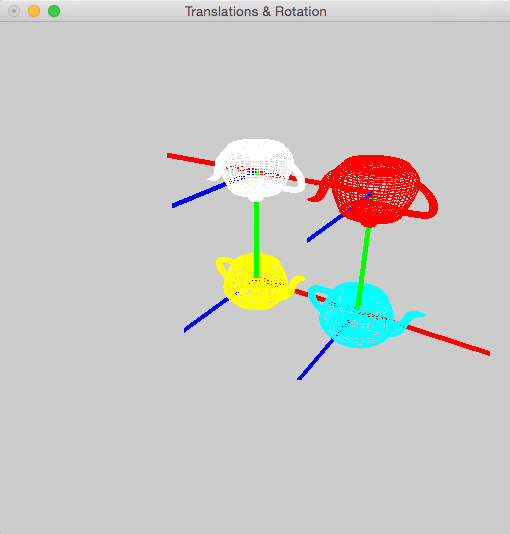
\includegraphics[height=7cm]{OGL_transform/localCoordXform.png}
    \caption{서로 다른 위치에 서로 다른 방향으로 놓인 주전자들}
    \label{fig:OGL_transform:localCoordXform}
\end{figure}

이제 이러한 문제를 다소 쉽게 접근할 수 있는 다른 방법을 사용해 보자. 이 방식은 물체의 변환이 아니라 좌표계의 변환으로 이해하는 것이다. 앞의 결과를 그릴 때에 각각의 주전자가 가진 지역 좌표계를 함께 그려보자. 그림 \ref{fig:OGL_transform:localCoordXform}에서 각각의 주전자는 길이가 0.5인 좌표축으로 표시된 지역좌표계가 붙어있다.
노란색 주전자는 아무런 변환 적용 없이 그린다. 따라서 전역 좌표계와 일치하는 지역 좌표계를 가지고 있다. 


\begin{verbatim}
glLoadIdentity();
draw(yellow);
\end{verbatim}

이제 하늘색 주전자를 그리려고 한다. 이 하늘색 주전자는 노란색 주전자의 좌표계에서 보았을 때 $x$ 축으로 1만큼 이동하여 있다. 따라서 다음과 같이 적용한다.

\begin{verbatim}
glTranslatef(1.0,0.0,0.0);
draw(cyan);
\end{verbatim}

다음으로 붉은 색 주전자를 보자. 이 주전자는 하늘색 주전자에서 $y$ 축으로 1만큼 올라간 뒤에, {\bf 이동된 좌표계}에서 $z$축을 기준으로 180도 회전한다. 따라서 다음과 같이 작성할 수 있다.

\begin{verbatim}
glTranslatef(0.0, 1.0, 0.0);
glRotatef(180, 0.0, 0.0, 1.0);
draw(red);
\end{verbatim}

그런데, 이 변환은 순서를 바꾸어 하늘색 주전자에서 $z$축 회전을 먼저 적용한 뒤에 $y$축 기준으로 -1만큼 이동하는 것과도 같다. 따라서 다음과 같이 적용해도 동일한 결과가 나온다.

\begin{verbatim}
glRotatef(180, 0.0, 0.0, 1.0);
glTranslatef(0.0, -1.0, 0.0);
draw(red);
\end{verbatim}

마지막으로 흰색 주전자는 붉은 색 주전자에서 $x$ 축으로 1만큼 이동한 것이므로 다음과 같이 코딩한다.

\begin{verbatim}
glTranslatef(1.0, 0.0, 0.0);
draw(white);
\end{verbatim}

이상과 같은 방법으로 변환을 이해하면 쉽게 다음 변환을 적용할 수 있을 것이다. 
코드 \ref{code:OGL_transform:rotation_translation}는 이러한 변환 적용을 구현한 예이다.

\begin{algorithmbis}[ 회전과 이동이 포함된 변환 적용 예]\label{code:OGL_transform:rotation_translation}
\lstset{language=C++, escapechar=^} 
\begin{lstlisting}
void drawLocalAxes() { drawAxes(); }
void draw() {    glutWireTeapot(0.3);}

void display() {

    ^{\sf [[카메라 설정과 버퍼 지우기 등의 코드]]}^

    drawLocalAxes();
    glColor4f(1, 1, 0, 0.25);
    draw();
    
    glTranslatef(1.0, 0.0, 0.0);
    drawLocalAxes();
    glColor4f(0, 1, 1, 0.25);
    draw();
    
    glRotatef(180, 0.0, 0.0, 1.0);
    glTranslatef(0.0,-1.0, 0.0);
    drawLocalAxes();
    glColor4f(1, 0, 0, 0.25);
    draw();
    
    glTranslatef(1.0, 0.0, 0.0);
    drawLocalAxes();
    glColor4f(1, 1, 1, 0.25);
    draw();
    
    glutSwapBuffers();
}

\end{lstlisting}
\end{algorithmbis}


\subsection{크기 변경이 포함된 경우}

지역좌표계의 변환 중심으로 생각하기는 이동과 회전이 복합적으로 이뤄질 때, 변환의 적용 결과가 어떻게 될 것인지를 쉽게 이해할 수 있도록 도와준다. 그런데, 크기 변경이 포함될 경우에는 문제가 생긴다.
다시 말해, 지역좌표계 변환을 통한 복합 변환의 이해는 강체(rigid) 변환에 대해서만 적용된다고 할 수 있다. 이를 예를 통해 살펴 보도록 하자.
다음의 그림 \ref{fig:OGL_transform:translateAndRot}과 같은 장면을 그리고 싶다고 하자. 각 변의 길이가 1인 정육면체가 있다. 이 정육면체의 크기를 바꿔 그림 \ref{fig:OGL_transform:translateAndRot}과 같이 높이 2, 너비 1, 깊이 1인 육면체로 만드려면 {\sf glScalef}와 같은 함수를 다음과 같이 사용하면 된다.

\begin{verbatim}
glScalef(1.0, 2.0, 1.0);
\end{verbatim}

\begin{figure}[h!]
  \centering
    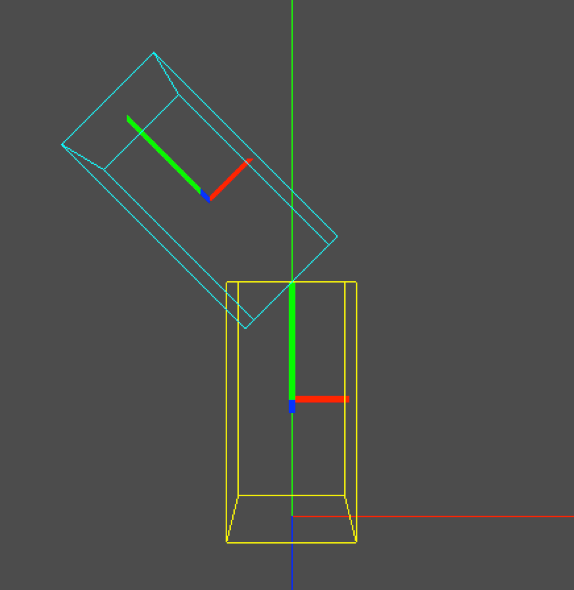
\includegraphics[height=7cm]{OGL_transform/noScale.png}
    \caption{동일한 육면체에 서로 다른 이동과 회전을 가하여 얻은 결과}
    \label{fig:OGL_transform:translateAndRot}
\end{figure}


이 육면체가 $xz$ 평면위에 놓이도록 하려면 $y$축 방향으로 0.5만큼만 움직이면 된다. 이때 0.5만 움직이는 것에 유의하라. 
이미 지역좌표계가 {\sf glScale}에 의해 변환되었기 때문에 0.5만 들어올려도 전역좌표계에서는 1만큼 올라가게 된다.
따라서 노란색 육면체는 다음과 같이 그릴 수 있다.

\begin{verbatim}
glScalef(1.0, 2.0, 1.0);		// S
glTranslatef(0.0, 0.5, 0.0);	// T1
draw(yellow);
\end{verbatim}


문제는 그 위에 있는 하늘색 육면체이다. 이 육면제는 노란색 육면체를 0.5만큼 들어올린 뒤에 z축 기준으로 회전을 시키고, 이렇게 변환된 공간에서 다시 y축 기준으로 0.5만큼 이동시키면 될 것으로 보인다. 즉 다음과 같은 변환 적용으로 구현이 가능할 것처럼 보인다.

\begin{verbatim}
glTranslatef(0.0, 0.5, 0.0);	// T2
glRotatef(45, 0.0, 0.0, 1.0);	// R
glTranslatef(0.0, 0.5, 0.0);	// T3
draw(cyan);
\end{verbatim}

그러나 실제로 이렇게 코딩을 하면 그림 \ref{fig:OGL_transform:translateAndRotWithScale}와 같은 결과를 얻는다. 이는 크기변경 변환 때문이다. 

\begin{figure}[h!]
  \centering
    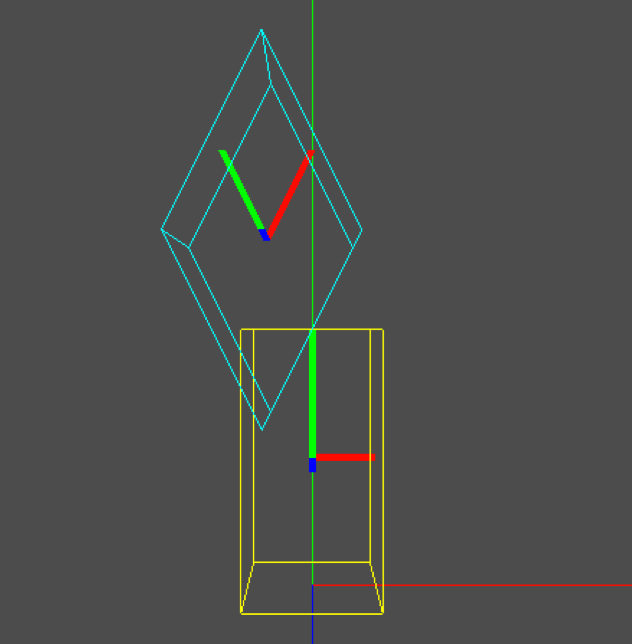
\includegraphics[height=7cm]{OGL_transform/scale.png}
    \caption{크기 변경에 의해 실제로 얻게 되는 모습}
    \label{fig:OGL_transform:translateAndRotWithScale}
\end{figure}

실제로 하늘색 육면체에 적용된 변환은 다음과 같다.

$${\mathbf S \mathbf T_1 \mathbf T_2 \mathbf R \mathbf T_3}$$

가장 마지막에 적용되는 ${\mathbf S}$는 전역 좌표계를 기준으로 크기변경이 일어나기 때문에 기울어진 하늘색 육면체의 방향(orientation)을 고려하지 않고 크기 변경이 이뤄진다. 따라서 위의 그림과 같이 육면체가 길쭉해지지 않고 대각선 방향으로 확대된 것이다.

이를 해결하는 방법은 행렬 스택 연산인 {\sf glPushMatrix()}와 {\sf glPopMatrix()}를 활용하여 크기변경 변환은 적용된 객체 이외에서 영향을 미치지 않도록 제한하는 것이다. 두 함수는 다음과 같은 일을 수행한다.\index{glPushMatrix}\index{glPopMatrix}

\begin{tabular}{|c|p{10cm}|}\hline
{\small \sf 함수명} & {\small \sf 역할}\\ \hline
{\small \sf glPushMatrix} & {\small \sf 현재의 CTM을 스택에 저장한다.}\\ \hline
{\small \sf glPopMatrix} & {\small \sf 행렬 스택을 pop하여 CTM을 갱신한다.}\\ \hline
\end{tabular}\\

따라서 {\sf glPushMatrix}를 수행한 뒤에 {\sf glPopMatrix}를 수행하면 직전의 {\sf glPushMatrix} 수행 당시의 CTM으로 복원이 된다. 이를 이용하여 육면체에 적용되는 크기 변경 변환의 영향 범위를 각 객체로 한정해 보자.

\begin{verbatim}
glTranslatef(0.0, 1.0, 0.0);
glPushMatrix();
glScalef(1.0, 2.0, 1.0);
draw(yellow);
glPopMatrix();
\end{verbatim}

여기서 주의할 것은 크기변경의 변환이 외부에 영향을 미치지 않고, {\sf glTranslatef}가 불릴 때는 크기 변경 변환에 의해 좌표계가 바뀌기 때문에 {\sf glTranslatef}에 사용된 이동량이 1이라는 것이다. 이것은 중심이 원점에 있는 단위 길이의 정육면체를 1만큼 이동 시킨 뒤에 $y$ 축 방향으로 2배 늘리면 아래 변이 $xz$ 평면에 닿기 때문이다. 
이제 하늘색 육면체를 그려보자. 이 육면체는 앞서 그린 노란색 육면체의 크기변경에 영향을 받지 않는다. 따라서 적당한 위치와 방향을 잡은 뒤에 다시 크기 변경을 적용해야 한다.

\begin{verbatim}
glTranslatef(0.0, 1.0, 0.0);
glRotatef(45, 0.0, 0.0, 0.0);
glTranslatef(0.0, 1.0, 0.0);
glPushMatrix();
glScalef(1.0, 2.0, 1.0);
draw(yellow);
glPopMatrix();
\end{verbatim}


이상의 작업이 완료되면 다음 그림 \ref{fig:OGL_transform:translateAndRot}과 같이 원하는 결과를 얻을 수 있다.



\section{계층적 모델링(hierarchical modeling)}\index{계층적 모델링}\index{hierarchical modeling}

컴퓨터 그래픽스로 표현하는 객체들 가운데 상당수의 것들은 구조를 가지고 있다. 이 구조는 인간이나 로봇과 같은 구조체에서 볼 수 있는 바와 같이 계층적(hierarchical) 특징을 가진 경우가 많다.

계층적 구조를 로봇의 예를 들어 살펴 보자. 인간형 로봇이 있다고 할 때, 이 로봇은 관절로 연결된 여러 개의 부분 요소로 나뉜다. 이 요소들은 루트가 있는 트리 구조로 표현할 수 있는데, 예를 들어 머리, 몸통, 위팔, 아래팔, 하박, 허벅지, 종아리로 구성되어 있다고 가정하면 몸통을 최상위 노드로 두고, 이 몸통의 자식 노드로 머리, 두 위팔, 두 허벅지를 달 수 있다. 그리고 두 위팔 각각에 하나씩의 아래팔이 달리며, 두 허벅지 각각에는 종아리가 하나씩 달릴 수 있다. 

각각의 노드는 부모 노드에 적용된 변환을 그대로 상속 받게 되는데, 이는 몸통이 움직이면 달린 모든 요소가 함께 움직여야 함을 의미한다. 반대로 자식 노드의 변환은 부모 노드에 영향을 미치지 못한다. 즉 종아리가 회전한다고 하여 몸통이나 허벅지가 움직이지는 않는 것이다. 이러한 방식으로 각각의 요소가 계층(階層)을 가지며
연결되어 있으며, 상위 계층의 변환에 그 자식 노드(node)가 영향을 받는 방식으로 구조체를 모델링하는 것을 계층적 모델링(hierarchical modeling)이라고 한다.

\begin{figure}[h!]
  \centering
    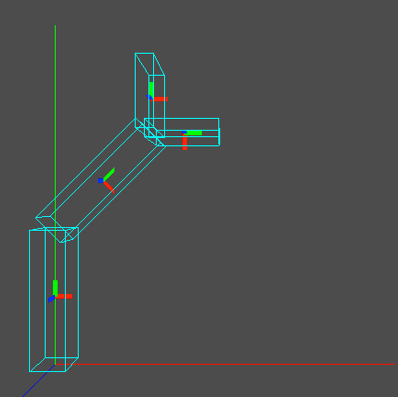
\includegraphics[height=7cm]{OGL_transform/robotArm.png}
    \caption{간단한 로봇 팔 모델의 예}
    \label{fig:OGL_transform:robotArm}
\end{figure}

계층적 모델링은 앞서 살펴본 {\sf glPushMatrix}와 {\sf glPopMatrix}를 활용하여 구현할 수 있다. 우선 그림 \ref{fig:OGL_transform:robotArm}와 같이 간단한 로봇 팔을 구현하여 보자. 이 로봇 팔인 두 개의 요소로 이루어진 팔이 이어져 있고, 그 끝에 갈라진 손이 달려 있는 모델이다.

이 모델은 다음과 같은 계층 구조로 볼 수 있다. 가장 아래쪽의 팔 하나에 기울어진 팔이 붙어 있고, 이 기울어진 팔에 두 개의 자식 노드, 즉 손을 구성하는 두 개의 요소가 같은 레벨(level)로 붙어 있는 것이다. 자식은 부모의 변환을 그대로 물려 받지만 형제(sibling) 노드들은 서로 영향을 미치면 안 된다. 

우선 팔 구성 요소는 길이가 4이며, 손을 구성하는 요소는 길이가 2라고 가정하자. 또한 팔 구성요소를 그리는 함수를 {\sf drawArm()}이라 하자.
그리고 손을 그리는 함수는 {\sf drawHand()}라고 하자. 처음으로 그려야 하는 루트(root) 객체인 가장 아래쪽 육면체는 다음과 같이 팔 요소의 길이 4를 고려하여 
그 반에 해당하는 2만큼 위로 올려서 그려야 한다.

\begin{verbatim}
glTranslatef(0.0, 2.0, 0.0);
drawArm();
\end{verbatim}

다음으로 45$^{\circ}$로 누워 있는 팔은 부모 노드의 변환을 반영해야 하므로 앞서 적용된 변환을 유지한 상태로 팔의 길이의 반만큼 올라간 뒤, 45도 회전하고, 나머지 반을 더 올라가서 끝을 맞춘다.

\begin{verbatim}
glTranslatef(0.0, 2.0, 0.0);
glRotatef(-45, 0.0, 0.0, 1.0);
glTranslatef(0.0, 2.0, 0.0);
drawArm();
\end{verbatim}

그리고 손을 그린다.  손 역시 비슷하게 작성할 수 있는데, 손의 길이가 2이므로 전체 길이의 반이 1이 된다는 점만 다르다.
우선 손의 중심을 팔의 끝에 두기 위해 팔의 길이 반에 해당하는 2만큼 이동시킨뒤 45$^{\circ}$ 회전하고, 손의 끝점을 관절부에 맞추기 위해 손의 길이 2의 반인 1만큼 이동하여 그림을 그린다.

\begin{verbatim}
glTranslatef(0.0, 2.0, 0.0);
glRotatef(-45, 0.0, 0.0, 1.0);
glTranslatef(0.0, 1.0, 0.0);
\end{verbatim}

이제 여기서 새로운 손 요소를 그리는 것이 쉽지 않다. 이 손은 방금 그린 손의 변환이 없다면 쉽게 마지막 팔 요소에 달 수 있다. 따라서 조금 전에 그린 손에 적용된 변환을 무효화하는 작업이 필요하다. 이런 작업은 무효화하여 돌아갈 시점의 변환이 기억되어 있다면 쉽게 가능한 일이다. 이를 위해서 {\sf glPushMatrix()}를 이용하여 돌아갈 지점의 변환상태를 스택에 저장해 두면 된다. 돌아가는 것은 어디서든 {\sf glPopMatrix()}를 부르면 된다. 따라서 앞의 코드는 다음과 같이 수정되어야 한다.

\begin{verbatim}
glPushMatrix();
glTranslatef(0.0, 2.0, 0.0); 
glRotatef(-45, 0.0, 0.0, 1.0);
glTranslatef(0.0, 1.0, 0.0);
glPopMatrix();
\end{verbatim}

다음으로 마지막 손 요소를 그리면 된다.

\begin{verbatim}
glTranslatef(0.0, 2.0, 0.0); 
glRotatef(45, 0.0, 0.0, 1.0);
glTranslatef(0.0, 1.0, 0.0);
\end{verbatim}

이상의 내용을 정리하면 코드 \ref{code:OGL_transform:robotArm}와 같다. 이 코드를 OpenGL 프로그램에
포함하여 실행하면 그림 \ref{fig:OGL_transform:robotArm}와 같은 모양을 얻을 수 있다.


\begin{algorithmbis}[계층적 구조로 로봇 팔 만들기]\label{code:OGL_transform:robotArm}
\lstset{language=C++, escapechar=^} 
\begin{lstlisting}
void drawArm() { // ^{\it 로봇 팔 그리기 코드. gl[Push$|$Pop]Matrix로 외부에 영향을 미치지 않음}^
    glPushMatrix();
    glScalef(1.0, 4.0, 1.0);
    glutWireCube(1.0);
    glPopMatrix();
}
void drawHand() { // ^{\it 로봇 손 그리기 코드. gl[Push$|$Pop]Matrix로 외부에 영향을 미치지 않음}^
    glPushMatrix();
    glScalef(1.0, 2.0, 1.0);
    glutWireCube(1.0);
    glPopMatrix();
}

void display() {
    glMatrixMode(GL_MODELVIEW);
    glLoadIdentity();
    gluLookAt(0, 0, 15, 0, 0, 0, 0, 1, 0);     // ^{\it 카메라의 위치를 설정하는 작업}^
    glClear(GL_COLOR_BUFFER_BIT|GL_DEPTH_BUFFER_BIT);
    
    // ^{\it 루트(root) 노드가 되는 팔을 하나 그리는 코드}^
    glTranslated(0.0, 2.0, 0.0);
    drawAxes();
    drawArm();
    // ^{\it 루트에 달린 두 번째 팔을 그리는 코드}^
    glTranslated(0.0, 2.0, 0.0);
    glRotatef(-45, 0.0, 0.0, 1.0);
    glTranslated(0.0, 2.0, 0.0);
    drawAxes();
    drawArm();
    // ^{\it 손을 그리기. 이때 사용한 변환이 다른 손에 영향을 미치지 않도록 gl[Push$|$Pop]Matrix 사용}^
    glPushMatrix();
    glTranslated(0.0, 2.0, 0.0);
    glRotatef(-45, 0.0, 0.0, 1.0);
    glTranslated(0.0, 1.0, 0.0);
    drawAxes();
    drawHand();
    glPopMatrix();
    // ^{\it 위의 glPushMatrix에 의해 현재 변환은 두 번째 팔을 그리고 난 상태와 동일함}^
    glTranslated(0.0, 2.0, 0.0);
    glRotatef(45, 0.0, 0.0, 1.0);
    glTranslated(0.0, 1.0, 0.0);
    drawAxes();
    drawHand();
    
    glutSwapBuffers();
}
\end{lstlisting}
\end{algorithmbis}

\subsection{가상의 태양계 만들기}
이제 이러한 계층적 모델링 기법을 이용하여 가상의 태양계를 만들어 보자. 이 가상의 태양계 중심에는 당연히 태양이 있다. 이 가상의 태양을 중심으로 가상의 수성, 금성, 지구, 화성, 목성이 존재한다고 하자. 가상의 지구는 하나의 위성을 가지고 있고, 목성은 세 개의 위성을 가지고 있다고 하자. 각각의 행성이나 위성은 태양 혹은 자신의 행성을 중심으로 공전해야 한다.  {\sf glPushMatrix}와 {\sf glPopMatrix}를 사용하면 이제 이러한 계층적 모델을 쉽게 구현할 수 있다. 이때 구를 그리기 위해 사용하고 있는 {\sf draw} 함수는
모두 4 개의 인자를 가지는데, 첫 번째 인자는 구의 반지름, 그리고 두 번재, 세 번째, 네 번째 인자는 구의 색을 결정하기 위한 RGB 채널 각각의 값이다.

\begin{algorithmbis}[가상의 태양계 만들기]\label{code:OGL_transform:solarSystem1}
\lstset{language=C++, escapechar=^} 
\begin{lstlisting}
void display() {
    static float t=10;     t+=1.0;
    ^{\sf [[카레라 설정, 버퍼 지우기, 중심 축 그리기 등을 수행]]}^
    
    draw(1, 1.0, 0.5, 0.0); //^{\it 태양}^
    
    glPushMatrix();
    glRotated(t, 0.0, 1.0, 0.0);
    glTranslated(3.0, 0.0, 0.0);
    draw(0.2, 0.5, 0.8, 1.0);  // ^{\it 수성}^
    glPopMatrix(); // ^{\it 수성 영향권 끝}^
    
    glPushMatrix();
    glRotated(t*1.5, 0.0, 1.0, 0.0);
    glTranslated(5.0, 0.0, 0.0);
    draw(0.2, 1.0, 1.0, 0.0); // ^{\it 금성}^
    glPopMatrix(); // ^{\it 금성 영향권 끝}^
    
    glPushMatrix();
    glRotated(t*0.8, 0.0, 1.0, 0.0);
    glTranslated(7.0, 0.0, 0.0);
    draw(0.2, 0.2, 0.2, 1.0); // ^{\it 지구}^
      glPushMatrix();
      glRotated(t*10.0, 0.0, 1.0, 0.0);
      glTranslated(0.5, 0.0, 0.0);
      draw(0.05, 1.0, 1.0, 1.0); // ^{\it 지구의 영향권 내에 달을 그림}^
      glPopMatrix(); // ^{\it 달의 영향권 끝}^
    glPopMatrix(); // ^{\it 지구의 영향권 끝}^

    glPushMatrix();
    glRotated(t*0.5, 0.0, 1.0, 0.0);
    glTranslated(10.0, 0.0, 0.0);
    draw(0.25, 1.0, 0.5, 0.4); // ^{\it 화성}^
    glPopMatrix(); // ^{\it 화성 영향권 끝}^

    glPushMatrix(); // ^{\it 목성 영향권의 시작}^
    glRotated(t*0.7, 0.0, 1.0, 0.0);
    glTranslated(14.0, 0.0, 0.0);
    draw(0.5, 1.0, 0.5, 0.4); // ^{\it 목성}^
     glPushMatrix();
      glRotated(t*10.0, 0.0, 1.0, 0.0);
      glTranslated(0.8, 0.0, 0.0);  
      draw(0.05, 1.0, 1.0, 1.0); // ^{\it 목성 위성 1번}^
      glPopMatrix(); // ^{\it 목성 위성 1번의 영향권 끝}^
      glPushMatrix();
      glRotated(t*12.0, 0.0, 1.0, 0.0);
      glTranslated(0.9, 0.0, 0.0);
      draw(0.07, 1.0, 1.0, 1.0); // ^{\it 목성 위성 2번}^
      glPopMatrix(); // ^{\it 목성 위성 2번의 영향권 끝}^
      glPushMatrix();
      glRotated(t*13.0, 0.0, 1.0, 0.0);
      glTranslated(0.7, 0.0, 0.0);
      draw(0.03, 1.0, 1.0, 1.0); // ^{\it 목성 위성 3번}^
      glPopMatrix(); //  ^{\it 목성 위성 2번의 영향권 끝}^
    glPopMatrix(); //  // ^{\it 목성의 영향권 끝}^
    
    glutSwapBuffers();
}

\end{lstlisting}
\end{algorithmbis}

\begin{figure}[h!]
  \centering
    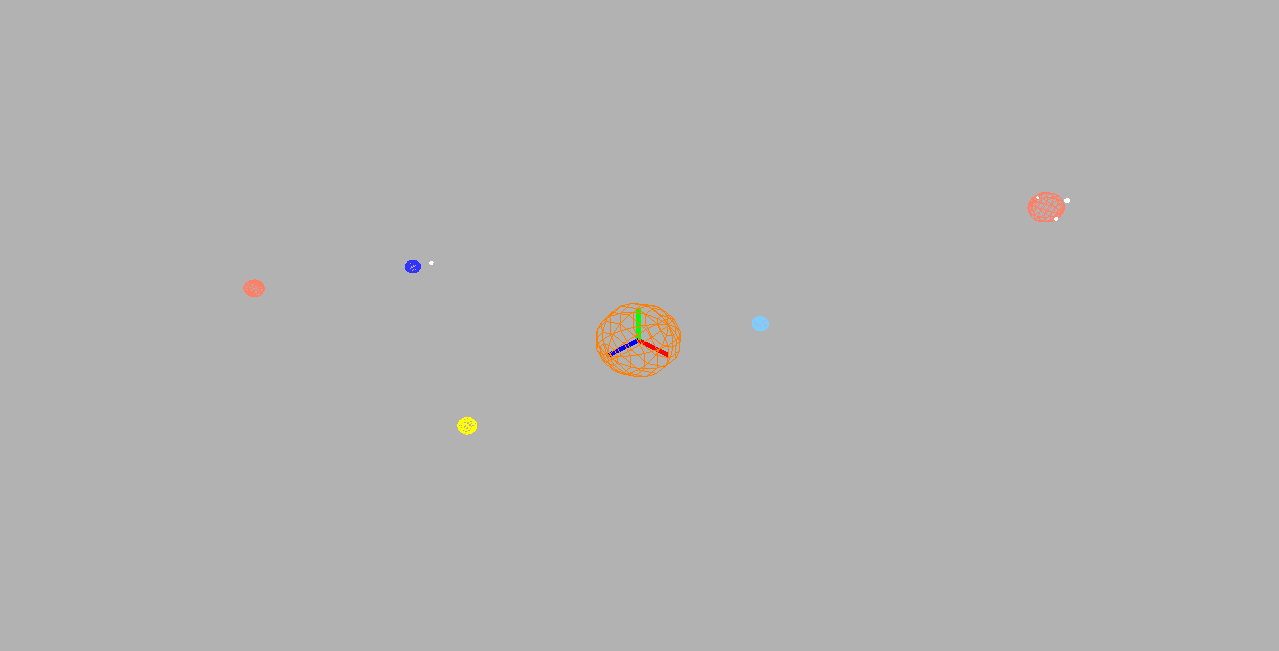
\includegraphics[height=6cm]{OGL_transform/solar1.png}
    \caption{태양을 중심으로 공전하는 가상 태양계}
    \label{fig:OGL_transform:solar1}
\end{figure}

이상의 코드를 이용하여 그림 \ref{fig:OGL_transform:solar1}와 같이 원점에 있는 태양의 주위를 도는 5 개의 행성이 공전을 하며, 이 중 두 개의 행성은 각각 1 개와 3 개의 위성을 가지고 있는 가상의 태양계를 만들 수 있다. 그런데, 이 코드를 개선하여 각 천체들이 움직이는 공전궤도를 표현하고 싶다면 어떻게 해야할까?
우리의 모델은 공전궤도가 원이다. 따라서 이 궤도들은 반지름이 다른 원들로 표현될 수 있다. 이런 원을 표현할 수 있는  drawCircle(radius)  함수를 다음과 같이 구현하자.

\begin{algorithmbis}[공전 궤도를 표현하는 원 그리기]\label{code:OGL_transform:circleDraw}
\lstset{language=C++} 
\begin{lstlisting}
void drawCircle(float radius) {
   glColor3f(1.0, 1.0, 1.0);
   glBegin(GL_LINE_LOOP);
   for (int i=0; i<50; i++) {
     glVertex3f(
            radius*cos(6.28*float(i)/50.0), 
            0.0, 
            radius*sin(6.28*float(i)/50.0));
   }
   glEnd();
}
\end{lstlisting}
\end{algorithmbis}

이제 이 함수가 언제 불려야 하는지를 결정해야 한다. 어떤 천체 궤도의 중심은 계층적 모델링 관점에서 보면 부모 노드의 위치에 해당한다. 따라서 태양을 중심으로 돌고 있는 수성, 금성, 지구, 화성, 목성의 궤도는 태양에 적용된 변환 단계에서 그려져야 한다. 마찬가지로 달의 궤도는 지구에 필요한 변환이 적용된 후 다른 변환이 적용되기 전에 지구와 달 사이의 거리에 해당하는 반지름으로 그리면 된다. 가상 목성의 세 가상 위성들의 궤도는 목성에 필요한 변환 적용후 각 위성이 목성에서 떨어진 거리만큼의 반지름을 가진 원을 그리면 된다. 따라서 다음과 같이 코드를 수정하면 궤도가 그려진 태양계 모델을 만들 수 있다. 결과는 그림 \ref{fig:OGL_transform:solar2}와 같다.

\begin{figure}[h!]
  \centering
    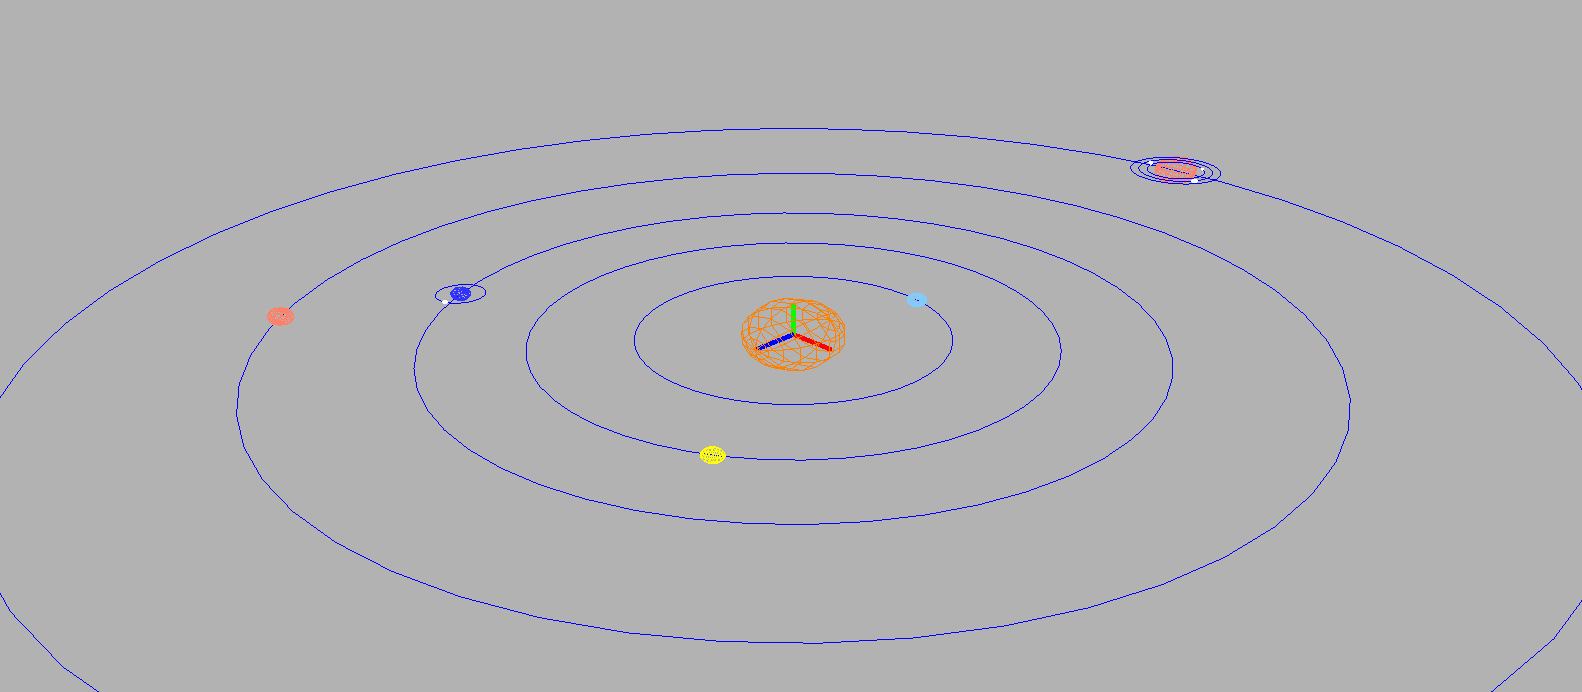
\includegraphics[height=6cm]{OGL_transform/solar2.png}
    \caption{공전 궤도를 그린 결과}
    \label{fig:OGL_transform:solar2}
\end{figure}


\begin{algorithmbis}[궤도를 포함한 태양계 모들 그리기]\label{code:OGL_transform:soloarSystem2}
\lstset{language=C++,escapechar=^} 
\begin{lstlisting}
    static float t=10;     t+=1.0;
    ^{\sf [[카레라 설정, 버퍼 지우기, 중심 축 그리기 등을 수행]]}^
    
    draw(1, 1.0, 0.5, 0.0); //^{\it 태양}^
    drawCircle(3.0); // ^{\it \color{red} 수성 궤도 그리기}^
    drawCircle(5.0); // ^{\it \color{red} 금성 궤도 그리기}^
    drawCircle(7.0); // ^{\it \color{red} 지구 궤도 그리기}^
    drawCircle(10.0);// ^{\it \color{red} 화성 궤도 그리기}^
    drawCircle(14.0);// ^{\it \color{red} 목성 궤도 그리기}^
    
    glPushMatrix();
      ^{\sf [[수성 변환과 그리기]]}^
    glPopMatrix(); // ^{\it 수성 영향권 끝}^
    
    glPushMatrix();
      ^{\sf [[금성 변환과 그리기]]}^
    glPopMatrix(); // ^{\it 금성 영향권 끝}^
    
    glPushMatrix();
      ^{\sf [[지구 변환과 그리기]]}^
      drawCircle(0.5); // ^{\it \color{red} 달의 궤도 그리기}^
      glPushMatrix();
      ^{\sf [[달의 변환과 그리기]]}^
      glPopMatrix(); // ^{\it 달의 영향권 끝}^
    glPopMatrix(); // ^{\it 지구의 영향권 끝}^
    
    glPushMatrix();
      ^{\sf [[화성 변환과 그리기]]}^
    glPopMatrix(); // ^{\it 화성 영향권 끝}^
    
    glPushMatrix(); // ^{\it 목성 영향권의 시작}^
      ^{\sf [[목성 변환과 그리기]]}^
      drawCircle(0.7); // ^{\it \color{red} 목성 위성 1의 궤도 그리기}^
      drawCircle(0.9); // ^{\it \color{red} 목성 위성 2의 궤도 그리기}^
      drawCircle(1.1); // ^{\it \color{red} 목성 위성 3의 궤도 그리기}^
      glPushMatrix();
        ^{\sf [[목성 위성 1의 변환과 그리기]]}^
      glPopMatrix(); // ^{\it 목성 위성 1번의 영향권 끝}^
      glPushMatrix();
        ^{\sf [[목성 위성 2의 변환과 그리기]]}^
      glPopMatrix(); // ^{\it 목성 위성 2번의 영향권 끝}^
      glPushMatrix();
        ^{\sf [[목성 위성 3의 변환과 그리기]]}^
      glPopMatrix(); //  ^{\it 목성 위성 2번의 영향권 끝}^
    glPopMatrix(); //  // ^{\it 목성의 영향권 끝}^
\end{lstlisting}
\end{algorithmbis}

